\documentclass[11pt,a4paper]{article}
\usepackage[margin=23mm,top=24mm,bottom=25mm,headheight=15pt]{geometry}
\usepackage[T1]{fontenc}
\usepackage[utf8]{inputenc}
\usepackage{mathpazo}
\usepackage[scaled=0.92]{helvet}
\usepackage{courier}
\DeclareUnicodeCharacter{2212}{\ensuremath{-}}
\DeclareUnicodeCharacter{2265}{\ensuremath{\ge}}
\DeclareUnicodeCharacter{2264}{\ensuremath{\le}}
\DeclareUnicodeCharacter{03A9}{\ensuremath{\Omega}}
\DeclareUnicodeCharacter{221A}{\ensuremath{\surd}}
\usepackage{microtype}
\usepackage[table]{xcolor}
\definecolor{Cosmic}{HTML}{26113F}
\definecolor{Purple}{HTML}{512575}
\definecolor{Muted}{HTML}{6B6274}
\definecolor{Gold}{HTML}{BB925A}
\definecolor{Pale}{HTML}{F4F0F7}
\usepackage{graphicx}
\setkeys{Gin}{keepaspectratio}
\usepackage{longtable,booktabs,array,calc}
\usepackage{amsmath,amssymb}
\usepackage{etoolbox}
\usepackage{enumitem}
\setlist{itemsep=0.25em,topsep=0.4em,leftmargin=1.6em}
\usepackage{titlesec}
\usepackage{needspace}
\titleformat{\section}{\sffamily\bfseries\Large\color{Purple}}{}{0em}{}
\titleformat{\subsection}{\sffamily\bfseries\large\color{Purple}}{}{0em}{}
\titleformat{\subsubsection}{\sffamily\bfseries\normalsize\color{Purple}}{}{0em}{}
\titlespacing*{\section}{0pt}{1.65em}{0.65em}
\titlespacing*{\subsection}{0pt}{1.2em}{0.45em}
\usepackage{fancyhdr}
\pagestyle{fancy}
\fancyhf{}
\fancyhead[L]{\sffamily\fontsize{8}{9}\selectfont\color{Muted}AGI ALPHA FLYWHEEL}
\fancyhead[R]{\sffamily\fontsize{8}{9}\selectfont\color{Muted}THE CERTIFIED BOUNDARY EDITION}
\fancyfoot[L]{\sffamily\fontsize{8}{9}\selectfont\color{Muted}RESEARCH REVIEW · 27 OCTOBER 2026}
\fancyfoot[R]{\sffamily\small\color{Purple}\thepage}
\renewcommand{\headrulewidth}{0.25pt}
\renewcommand{\footrulewidth}{0pt}
\usepackage{caption}
\captionsetup{font=small,labelfont={bf,sf},textfont=it,skip=7pt}
\usepackage{float}
\usepackage{tikz}
\usepackage{fvextra}
\usepackage{color}
\usepackage{fancyvrb}
\newcommand{\VerbBar}{|}
\newcommand{\VERB}{\Verb[commandchars=\\\{\}]}
\DefineVerbatimEnvironment{Highlighting}{Verbatim}{commandchars=\\\{\}}
% Add ',fontsize=\small' for more characters per line
\newenvironment{Shaded}{}{}
\newcommand{\AlertTok}[1]{\textcolor[rgb]{1.00,0.00,0.00}{\textbf{#1}}}
\newcommand{\AnnotationTok}[1]{\textcolor[rgb]{0.38,0.63,0.69}{\textbf{\textit{#1}}}}
\newcommand{\AttributeTok}[1]{\textcolor[rgb]{0.49,0.56,0.16}{#1}}
\newcommand{\BaseNTok}[1]{\textcolor[rgb]{0.25,0.63,0.44}{#1}}
\newcommand{\BuiltInTok}[1]{\textcolor[rgb]{0.00,0.50,0.00}{#1}}
\newcommand{\CharTok}[1]{\textcolor[rgb]{0.25,0.44,0.63}{#1}}
\newcommand{\CommentTok}[1]{\textcolor[rgb]{0.38,0.63,0.69}{\textit{#1}}}
\newcommand{\CommentVarTok}[1]{\textcolor[rgb]{0.38,0.63,0.69}{\textbf{\textit{#1}}}}
\newcommand{\ConstantTok}[1]{\textcolor[rgb]{0.53,0.00,0.00}{#1}}
\newcommand{\ControlFlowTok}[1]{\textcolor[rgb]{0.00,0.44,0.13}{\textbf{#1}}}
\newcommand{\DataTypeTok}[1]{\textcolor[rgb]{0.56,0.13,0.00}{#1}}
\newcommand{\DecValTok}[1]{\textcolor[rgb]{0.25,0.63,0.44}{#1}}
\newcommand{\DocumentationTok}[1]{\textcolor[rgb]{0.73,0.13,0.13}{\textit{#1}}}
\newcommand{\ErrorTok}[1]{\textcolor[rgb]{1.00,0.00,0.00}{\textbf{#1}}}
\newcommand{\ExtensionTok}[1]{#1}
\newcommand{\FloatTok}[1]{\textcolor[rgb]{0.25,0.63,0.44}{#1}}
\newcommand{\FunctionTok}[1]{\textcolor[rgb]{0.02,0.16,0.49}{#1}}
\newcommand{\ImportTok}[1]{\textcolor[rgb]{0.00,0.50,0.00}{\textbf{#1}}}
\newcommand{\InformationTok}[1]{\textcolor[rgb]{0.38,0.63,0.69}{\textbf{\textit{#1}}}}
\newcommand{\KeywordTok}[1]{\textcolor[rgb]{0.00,0.44,0.13}{\textbf{#1}}}
\newcommand{\NormalTok}[1]{#1}
\newcommand{\OperatorTok}[1]{\textcolor[rgb]{0.40,0.40,0.40}{#1}}
\newcommand{\OtherTok}[1]{\textcolor[rgb]{0.00,0.44,0.13}{#1}}
\newcommand{\PreprocessorTok}[1]{\textcolor[rgb]{0.74,0.48,0.00}{#1}}
\newcommand{\RegionMarkerTok}[1]{#1}
\newcommand{\SpecialCharTok}[1]{\textcolor[rgb]{0.25,0.44,0.63}{#1}}
\newcommand{\SpecialStringTok}[1]{\textcolor[rgb]{0.73,0.40,0.53}{#1}}
\newcommand{\StringTok}[1]{\textcolor[rgb]{0.25,0.44,0.63}{#1}}
\newcommand{\VariableTok}[1]{\textcolor[rgb]{0.10,0.09,0.49}{#1}}
\newcommand{\VerbatimStringTok}[1]{\textcolor[rgb]{0.25,0.44,0.63}{#1}}
\newcommand{\WarningTok}[1]{\textcolor[rgb]{0.38,0.63,0.69}{\textbf{\textit{#1}}}}
\DefineVerbatimEnvironment{Highlighting}{Verbatim}{breaklines,commandchars=\\\{\},fontsize=\small}
\usepackage{xurl}
\usepackage[colorlinks=true,linkcolor=Purple,urlcolor=Purple,citecolor=Purple,breaklinks=true]{hyperref}
\hypersetup{pdftitle={AGI ALPHA FLYWHEEL --- When Capability Creates
Opportunity — The Certified Boundary Edition},pdfauthor={Vincent Boucher — President of MONTREAL.AI},pdfsubject={Exact covering-system certificates, conventional challenge and complete conditional economics},pdfkeywords={covering systems, exact certificate, AGI ALPHA, research review}}
\urlstyle{same}
\Urlmuskip=0mu plus 2mu
\renewcommand{\texttt}[1]{{\ttfamily\small #1}}
\setlength{\parindent}{0pt}
\setlength{\parskip}{0.45em}
\renewcommand{\baselinestretch}{1.07}
\setlength{\emergencystretch}{2em}
\setlength{\tabcolsep}{5pt}
\renewcommand{\arraystretch}{1.18}
\AtBeginEnvironment{longtable}{\small}
\providecommand{\tightlist}{\setlength{\itemsep}{0pt}\setlength{\parskip}{0pt}}
\providecommand{\passthrough}[1]{#1}
\newcommand{\pandocbounded}[1]{#1}
\newlength{\cslhangindent}
\setlength{\cslhangindent}{1.5em}
\newlength{\csllabelwidth}
\setlength{\csllabelwidth}{3em}
\newenvironment{CSLReferences}[2]{\begingroup\small\raggedright\setlength{\parskip}{0.5em}\setlength{\parindent}{0pt}}{\endgroup}
\newcommand{\CSLBlock}[1]{#1\hfill\break}
\newcommand{\CSLLeftMargin}[1]{\parbox[t]{\csllabelwidth}{#1}}
\newcommand{\CSLRightInline}[1]{\parbox[t]{\linewidth-\csllabelwidth}{#1}\break}
\newcommand{\CSLIndent}[1]{\hspace{\cslhangindent}#1}
\newcommand{\evidencebreak}{\clearpage}
\begin{document}
\begin{titlepage}
\pagecolor{Cosmic}\color{white}
\begin{tikzpicture}[remember picture,overlay]
\draw[white,opacity=.08,line width=.6pt] ([xshift=35mm,yshift=-65mm]current page.north east) circle (78mm);
\draw[Gold,opacity=.35,line width=.5pt] ([xshift=-28mm,yshift=-65mm]current page.north east) circle (54mm);
\draw[white,opacity=.12,line width=.5pt] ([xshift=-28mm,yshift=-65mm]current page.north east) circle (73mm);
\foreach \x/\y/\r in {15/17/.8,37/43/.5,71/22/.6,109/55/.7,154/31/.6,172/82/.9,34/101/.5,126/97/.5,188/133/.6,29/166/.6,155/186/.7,58/217/.5,177/235/.5,102/262/.7}
  \fill[white,opacity=.28] ([xshift=\x mm,yshift=-\y mm]current page.north west) circle (\r pt);
\end{tikzpicture}
{\sffamily\small\color{Gold}MONTREAL.AI\hfill RESEARCH REVIEW / 2026}\par
\vspace{20mm}
{\sffamily\fontsize{14}{18}\selectfont\color{Gold}THE CERTIFIED BOUNDARY EDITION}\par
\vspace{6mm}
{\sffamily\bfseries\fontsize{33}{37}\selectfont AGI ALPHA\\ FLYWHEEL}\par
\vspace{5mm}
{\sffamily\fontsize{23}{28}\selectfont When Capability\\Creates Opportunity}\par
\vspace{8mm}
{\fontsize{13}{18}\selectfont Transformational Intelligence,\\Experience-Trained Specialists and the\\Expanding Frontier of Profitable Work}\par
\vspace{10mm}
\textcolor{Gold}{\rule{35mm}{0.8pt}}\par
{\sffamily\fontsize{14}{19}\selectfont An executable answer to a\\covering-system question}\par
\vspace{8mm}
{\fontsize{19}{24}\selectfont \(h\ge\dfrac{17902560}{18258529}>0.98\)}\par
{\sffamily\small Exact proof · Independent checking · Honest economics}\par
\vfill
{\sffamily\bfseries\large Vincent Boucher}\par
{\sffamily\normalsize President of MONTREAL.AI}\par
\vspace{6mm}
{\sffamily\fontsize{8.5}{11}\selectfont TRANSFORMATIONAL INTELLIGENCE: LEARNING TO CHANGE THE GAME}\par
{\sffamily\fontsize{10}{13}\selectfont\color{Gold}FIND YOUR ALPHA. BUILD YOUR SUCCESSOR \(\Omega\).}\par
\vspace{4mm}
{\sffamily\small 27 October 2026 · Research-review edition v1}\par
\end{titlepage}
\nopagecolor\color{black}
\setcounter{page}{1}
\Needspace{9\baselineskip}

\hypertarget{a-question-that-now-has-a-checkable-answer}{%
\section{A question that now has a checkable
answer}\label{a-question-that-now-has-a-checkable-answer}}

\textbf{An unbounded search has become a finite, reusable proof.} This
study constructs an exact mathematical certificate that rules out a
proposed family of low-heft congruence partitions for every interval
length. A reader can check the result with ordinary Python, without a
language model, a numerical optimizer, a wallet or a trusted prediction
about future capability. The artifact is the useful outcome: a precise
answer that subsequent researchers can inspect, challenge and build
upon.

The problem is simple to state. Partition the integers from \(1\) to
\(n\) into complete residue classes, with each class containing at least
two integers of that interval. A class with modulus \(m\) contributes
\(1/m\) to the partition's \textbf{heft}. Gerry Myerson asks whether,
with distinct moduli, such a partition can have heft below \(0.98\)
(\protect\hyperlink{ref-myerson2026}{Myerson 2026};
\protect\hyperlink{ref-myerson2009}{Myerson, Poon, and Simpson 2009}).
We establish the following computer-assisted theorem:

\begin{samepage}

\[
\boxed{\displaystyle h=\sum_i\frac{1}{m_i}\ge
J:=\frac{17902560}{18258529}
=0.9805039606421744\ldots>0.98.}
\]

\end{samepage}

The strongest certificate was discovered by the fresh conventional
challenge and strengthened by exact normalization in independent review.
The proof covers every positive integer \(n\) admitting a partition and
even permits repeated moduli. It preserves complete residue classes,
exact coverage and at least two hits per class. It does not apply to
arbitrary selected arithmetic progressions, singleton classes or
two-dimensional coverings. The inspected prior general lower bound is
\(\sqrt8-2\approx0.828427\), from Emanuel's dissertation, Appendix C,
Theorem C.1 (\protect\hyperlink{ref-emanuel2011}{Emanuel 2011}). The
constant above is certified, not claimed optimal. A bounded literature
audit did not locate this result; external mathematical review and a
fuller priority assessment remain pending.

The enterprise conclusion is narrower than the scientific result. No
customer bought the work; actual revenue and receipts are zero, and
complete actual authoring cost is unknown. An explicit planning model
for review and integration of this existing artifact is conditionally
profitable with four compatible sponsors, but demand is unvalidated and
financing is required. A competent conventional shared arrangement has
the same economics. No measured Operational Alpha, superhuman
specialist, profitable skill compounding or general discovery engine is
established.

\textbf{Abstract.} We investigate whether a bounded, independently
challenged discovery process can produce a new useful result rather than
an architectural proposal or an attractive scenario. A diverse
opportunity screen rejects generic novelty claims already addressed by
established methods. A first exact-code construction lane fails to
improve the strongest located comparators. A subsequent finite-cover
investigation first constructs an exact degree-20 dual weight. A fresh
conventional challenge independently discovers a simpler
piecewise-linear weight; normalization by its exactly checked maximum
gives the stronger final bound. Two separately implemented
line-arrangement checkers and an analytic tail certify every allowed
class, while cell integrals transfer the result to every finite interval
length. Fresh tests examine additional classes, scope decisions and
malformed or altered inputs. The earlier polynomial proof remains
independently verified and reproducible. Failed numerical evidence is
retained. Existing AGI ALPHA provenance and execution components are
exercised locally without minting, live identity claims or financial
activity. Complete conditional accounting separates operating surplus,
full-project profit, funding needs, restricted deposits and service
obligations. The result demonstrates a portable research capability and
a concrete mathematical advance relative to inspected prior bounds. It
does not demonstrate an exclusive algorithmic advantage or a
commercially validated enterprise.

\begin{figure}
\centering
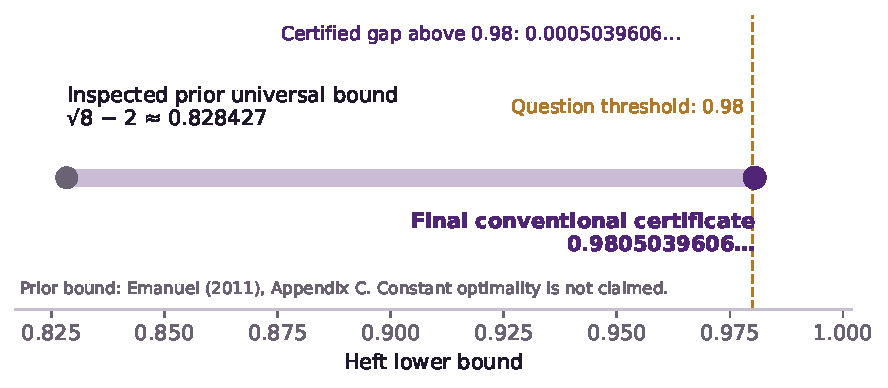
\includegraphics[width=0.95\textwidth,height=\textheight]{figures/bound.pdf}
\caption{The certified constant crosses the requested threshold. This is
a comparison with the strongest general bound located in the inspected
primary sources, not a universal priority or optimality claim.}
\end{figure}

\Needspace{9\baselineskip}

\hypertarget{discovering-the-opportunity}{%
\section{Discovering the
opportunity}\label{discovering-the-opportunity}}

\Needspace{7\baselineskip}

\hypertarget{purpose-before-application}{%
\subsection{Purpose before
application}\label{purpose-before-application}}

The motivating opportunity was to make a consequential unanswered
question yield an inspectable answer under available digital resources.
The study did not begin with a prescribed customer workflow. It searched
for targets with an external specification, an identifiable limitation,
a strong conventional challenge, a plausible beneficiary and a decisive
experiment. Mathematical construction became a viable lane because its
first useful output can be checked digitally and its acceptance need not
depend on a physical prototype or an unavailable archive.

For the selected problem, the limitation statement is:

\begin{quote}
Existing finite enumeration and finite integer-programming searches that
find no qualifying cover cannot rule out one at a larger interval
length: a cutoff leaves infinitely many lengths unresolved. An explicit
universal weight certificate resolves that remaining possibility while
preserving complete classes, exact partitioning and minimum class size.
A finite search could, of course, settle existence by finding a valid
witness.
\end{quote}

This statement concerns the insufficiency of a finite search as a
universal proof. It does not claim that conventional mathematics, an
existing university or a research organization lacks the ability to
discover such a proof. Duality, polynomial approximation and Bernstein
verification are established tools. The scientific contribution is the
explicit witness and resulting theorem.

The immediate beneficiary is the research community studying covering
systems. A separate possible buyer could commission reproducibility,
qualified review or integration of a fixed certificate. The former is a
demonstrated intellectual use; the latter is a commercial hypothesis. We
did not establish that the theorem has a near-term industrial
application or that a particular organization is unable to perform this
work.

\Needspace{7\baselineskip}

\hypertarget{a-small-diverse-screen-and-its-conventional-challenges}{%
\subsection{A small, diverse screen and its conventional
challenges}\label{a-small-diverse-screen-and-its-conventional-challenges}}

Six directions formed the initial screen. The detailed limitation
statements and primary-source comparisons are in the evidence package.

\textbf{Decision-directed experimental instruments.} The proposed
instrument would choose tests that settle a useful property without
identifying an entire model. Decision Region Determination and Hyperedge
Cutting already target that distinction, while exact dynamic programming
is practical on small finite cases
(\protect\hyperlink{ref-javdani2014}{Javdani et al. 2014}). The generic
mechanism did not survive the prior-art challenge.

\textbf{Combining incomplete causal evidence.} The proposed
representation would return sharp intervention bounds and extremal
compatible worlds from partial observations. Automated partial
identification already supplies this core mechanism
(\protect\hyperlink{ref-duarte2024}{Duarte et al. 2024}). A convenient
compiler alone would not establish a new productive possibility.

\textbf{Combining specialists without training data.} The proposal
sought transferable capability by aligning and merging networks.
Data-free, cycle-consistent model merging is direct prior art
(\protect\hyperlink{ref-crisostomi2024}{Crisostomi et al. 2024}). A new
label or a successful merge would not establish economic Alpha or a
stronger accepted outcome.

\textbf{Runtime enforcement.} The proposed component would preserve
useful action while blocking violations of a formal specification.
Shield synthesis is an established construction
(\protect\hyperlink{ref-bloem2015}{Bloem et al. 2015}). A new
implementation was insufficient for the flagship criterion.

\textbf{Exact zero-error communication codes.} This lane had a concrete
improvement target and independent digital verification. Strong
published witnesses, MILP, local search and straightforward compositions
were admitted. The executed searches reproduced known constructions but
did not improve them. We stopped the record-improvement claim rather
than changing the channel or weakening the comparator
(\protect\hyperlink{ref-itty2026}{Itty et al. 2026};
\protect\hyperlink{ref-buys2026}{Buys, Polak, and Zuiddam 2026};
\protect\hyperlink{ref-tandon2026}{Tandon 2026}).

\textbf{Finite residue partitions.} The public question supplied a fixed
threshold and clear original requirements. Finite exact-cover search was
attempted first. Its failure to find a witness suggested, without
proving, a lower-bound direction. A certificate that applies uniformly
to all lengths became the surviving research target
(\protect\hyperlink{ref-myerson2026}{Myerson 2026}).

Additional scouting considered quantum-code and small-design records.
Those screens did not produce a new accepted witness and are preserved
as exploratory notes. Screening conclusions are literature judgments,
not executed capability benchmarks.

\Needspace{7\baselineskip}

\hypertarget{why-this-became-feasible-in-this-study}{%
\subsection{Why this became feasible in this
study}\label{why-this-became-feasible-in-this-study}}

The changed arrangement combines an accessible, recently refreshed
public question; explicit computational definitions and prior examples;
interactive frontier-model reasoning; inexpensive standard optimization;
and exact independent verification. The 2026 public updates make the
outstanding threshold easy to identify without inventing a benchmark.
They do not make the mathematical question new
(\protect\hyperlink{ref-myerson2026}{Myerson 2026}). No unique
instrument unavailable to other organizations is claimed.

The useful representational move is from ``find a cover at larger
\(n\)'' to ``find one weight function that prices every permissible
class.'' A finite search can miss a distant witness. A valid universal
weight converts the same original question into finitely checkable
polynomial obligations plus a mathematical tail argument. This is a
change in what the particular completed artifact establishes, not a
claim that dual certificates were invented here.

\Needspace{9\baselineskip}

\hypertarget{the-construction-and-its-verification}{%
\section{The construction and its
verification}\label{the-construction-and-its-verification}}

\Needspace{7\baselineskip}

\hypertarget{a-weight-that-every-class-must-respect}{%
\subsection{A weight that every class must
respect}\label{a-weight-that-every-class-must-respect}}

\begin{samepage}

Let \(W\) be the continuous piecewise-linear function with knots
\(r/20\), \(r=0,\ldots,20\). Its first eleven heights are

\[0,159,316,493,721,981,1240,1500,1658,1818,1858,\]

\end{samepage}

\begin{samepage}

and the rest are their reflection about the midpoint. Extend it by zero
outside the interval. Its exact integral is \(A=1963/2\). The
construction proves that every complete progression with spacing \(d\)
and at least two points in \([0,1]\) obeys

\[d\sum_j W(a+jd)\le M:=\frac{18258529}{18240}.\]

\end{samepage}

Assign integer \(i\) the \textbf{cell integral}
\(w_i=\int_{(i-1)/n}^{i/n}W(x)\,dx\). Integrating the progression
inequality over the phase within each cell proves
\(m\sum_{i\in C}w_i\le M\) for every complete restricted class \(C\) of
modulus \(m\). Since the classes partition all integers exactly once,
\(A\le Mh\). Thus \(h\ge A/M=J\). This uses actual finite cells; it
introduces no limiting approximation or exception for small lengths.

\begin{figure}
\centering
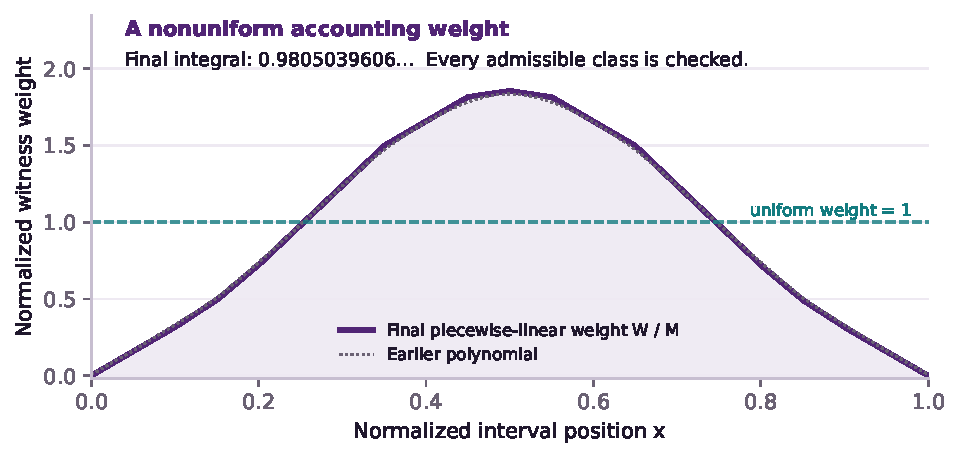
\includegraphics[width=0.95\textwidth,height=\textheight]{figures/witness.pdf}
\caption{The final piecewise-linear weight divided by its exact class
maximum, with the earlier polynomial shown for comparison. These curves
explain the construction; sampled plotting values do not certify it.}
\end{figure}

\begin{samepage}

For a class with \(k\) points, spacing \(d\) and first point \(a\), the
complete-class parameter domain is the quadrilateral

\[0\le a\le d,\qquad a+(k-1)d\le1\le a+kd.\]

\end{samepage}

Knot-crossing lines partition that quadrilateral into cells. Within a
cell, the class sum has the form \(A_1ad+B_1d^2+C_1d\). A maximum occurs
on a cell boundary: a nonzero mixed coefficient makes the Hessian
indefinite; when it is zero, the value is independent of \(a\) and
extends to a boundary. On each boundary segment, exact quadratic
maximization checks endpoints and any interior stationary point. All
knot lines and all four exterior boundaries are included.

The primary conventional checker examines 1,967 segments for
\(k=2,\ldots,20\) and obtains exact maximum \(M\). A separately written
checker reconstructs the clipping from polygon-edge intersections and
uses direct interpolation to fit the quadratic on every segment. It
agrees. For \(k\ge21\), the total variation of the derivative of the
zero extension is 21,200, yielding the universal tail bound
\(7905/8<M\). Appendix A gives the full proof.

\Needspace{7\baselineskip}

\hypertarget{independent-checking-and-fresh-confirmation}{%
\subsection{Independent checking and fresh
confirmation}\label{independent-checking-and-fresh-confirmation}}

The final certificate therefore rests on two distinct exact
implementations, a boundary-maximization lemma, an analytic tail and a
cell-average transfer argument. Independence means separate
implementations and derivations within the same AI-assisted study; it is
not independent institutional or human peer review. The accepted
relation at \(J\) is \textbf{greater than or equal to}. Strictness at
that exact constant is not claimed; strictness above \(0.98\) follows
because \(J>0.98\).

\begin{longtable}[]{@{}
  >{\raggedright\arraybackslash}p{(\columnwidth - 4\tabcolsep) * \real{0.3333}}
  >{\raggedright\arraybackslash}p{(\columnwidth - 4\tabcolsep) * \real{0.3333}}
  >{\raggedright\arraybackslash}p{(\columnwidth - 4\tabcolsep) * \real{0.3333}}@{}}
\toprule\noalign{}
\begin{minipage}[b]{\linewidth}\raggedright
Obligation
\end{minipage} & \begin{minipage}[b]{\linewidth}\raggedright
Executed evidence
\end{minipage} & \begin{minipage}[b]{\linewidth}\raggedright
Meaning
\end{minipage} \\
\midrule\noalign{}
\endhead
\bottomrule\noalign{}
\endlastfoot
Classes with 2--20 hits & All exact segment maxima agree in two
implementations & Entire parameter domains, including all boundary
edges \\
Classes with at least 21 hits & Exact tail \(7905/8<M\) & No class-size
cutoff remains \\
Every interval length & Exact cell-integral argument & No midpoint
approximation or finite-\(n\) extrapolation \\
Full final wrapper & Both exact verifiers recomputed in 1.55 seconds in
one local run & Local research verification, not a speed benchmark \\
Earlier polynomial certificate & 78/78 patches in both implementations;
exact all-length objective & A separate valid, weaker construction \\
Earlier fresh tests & 512 classes, four new lengths, 19 scope decisions
and 13 altered-input controls & Confirmation of the earlier artifact,
not evidence silently reassigned to the final one \\
\end{longtable}

For the final piecewise-linear certificate, a new frozen seed
(\texttt{202610274852}) generated 512 complete classes: 256 short
classes and 256 longer classes. Direct phase evaluations and exact
cell-integral inequalities all pass; cell weights telescope at nine
fresh interval lengths. Two deliberately invalid mathematical variants
are rejected. After correcting the JSON-null interface error, a separate
final audit recomputed the stronger proof in 1.49 seconds, matched 22/22
scope decisions, and refused all 21 specified isolated CLI controls. One
missing-helper case exits with an import error rather than structured
refusal; it produces no acceptance. These cases are implementation
checks, not a statistical substitute for proof or a model benchmark.

The final wrapper validates the requested scope, matches frozen source
bytes and recomputes the proof in an isolated directory. It does not
accept a result from an archived success flag. It refuses altered or
missing proof inputs, stronger unsupported bounds and strictness at the
exact final constant. Its hashes are reproducibility controls, not
signatures proving scientific correctness or ownership. Both research
wrappers refuse optimized Python because some underlying checkers use
assertions.

The earlier polynomial remains useful independent evidence. Its exact
coefficient file, both continuous-domain implementations, analytic tail
and all-length identity are preserved in Appendix B and the package. Its
bound \(h>I=0.9804028583156853\ldots\) is weaker than the final
conventional certificate. Its 512 fresh class tests used seed
\texttt{202610274850}, lengths up to one million and complete classes
under a frozen protocol; new midpoint lengths were 251, 257, 509 and
601. These finite checks confirm implementation behavior and do not
substitute for either universal proof.

\Needspace{7\baselineskip}

\hypertarget{the-failure-that-changed-the-result}{%
\subsection{The failure that changed the
result}\label{the-failure-that-changed-the-result}}

The first degree-20 numerical candidate had integral approximately
\(0.98558247\) and appeared stronger on a coarse grid. It was invalid.
Continuous exploration exposed a violation; independent exact checking
found an integer realization at \(n=26\), modulus 15, residue 11, with
class \(\{11,26\}\). Its normalized constraint value is approximately
\(1.046411318>1\). That candidate is rejected in the publication and
remains in the evidence package.

Dense constraints and eight cutting-plane iterations produced the
replacement. Decimal coefficients were converted to exact rationals and
scaled by \(2499/2500\) before certification. The frozen JSON still says
\texttt{UNVERIFIED}, reflecting its state when selected; later
acceptance receipts establish verification without rewriting the
candidate's identity. Two implementation errors in the all-length
refinement were also caught: accidental floor division of rational
expressions, and an attempted positivity interval larger than the
discrete-length argument required. Both original attempts and their
corrections are retained. Final adverse testing also caught an interface
error: an explicitly supplied JSON-null request was treated as an
omitted request. The mathematical proof still ran correctly, but the
schema refusal was wrong. The final interface was corrected and
refrozen; the failing code and receipt remain archived.

\Needspace{7\baselineskip}

\hypertarget{what-the-conventional-challenge-does-and-does-not-show}{%
\subsection{What the conventional challenge does and does not
show}\label{what-the-conventional-challenge-does-and-does-not-show}}

Nineteen conventional finite-cover runs produced seventeen valid
incumbents and no cover below 0.98; their aggregate recorded wall time
was 146.46 seconds. Two runs ended without an incumbent. A feasible
incumbent is not an optimum certificate, and none of these finite
searches establishes an all-length impossibility result.

The execution comparison gives ordinary methods the discovered
formulation, exact witness, proof and checker. They can reproduce the
same accepted result. This equality prevents an exclusive solver claim.
It does not erase the mathematical consequence of a previously
unrecorded explicit certificate.

\textbf{The strongest conventional challenge succeeds.} The fresh
workstream received the public question, primary references, ordinary
libraries and the same available tool permissions, without seeing the
polynomial witness. Standard finite LP duals suggested its
piecewise-linear construction. Its final exact certificate was completed
at 22:23:45 UTC, 4 minutes 36 seconds after the recorded start. Recorded
deliberate numerical work was approximately 145.9 CPU seconds, plus an
interrupted setup lasting less than six wall seconds whose CPU usage was
not captured.

The challenger initially used the convenient scale \(2003/2\), proving
\(h\ge1963/2003>0.98\). Its own exact maximum was smaller. Independent
audit used that maximum without changing any heights or useful
requirements, yielding the stronger \(J\). Reporting only the looser
scale would understate the conventional result. The conventional
construction meets the original target and exceeds the first polynomial
bound. We therefore stop any claim of exclusive superiority for that
first approach and publish the strongest joint scientific result.

This is a new explicit certificate relative to the inspected prior
sources, produced using established techniques. It does not establish a
new optimization method, an advantage from specialist retention, or a
reason an existing organization could not produce it.

Discovery must be assessed separately. The main opportunity search was
adaptive and exploratory. It was not a randomized, identical-information
comparison of ordinary and expert model use. A targeted fresh-context
conventional challenge was launched after the mathematical question had
been selected, with a ten-minute wall ceiling and 300 CPU-second
numerical-search ceiling. Its initial information and search are
retained separately. That experiment cannot establish population-level
discovery advantage or prove that humans or ordinary agents could not
find the result.

\Needspace{9\baselineskip}

\hypertarget{building-an-economic-possibility-around-a-useful-artifact}{%
\section{Building an economic possibility around a useful
artifact}\label{building-an-economic-possibility-around-a-useful-artifact}}

\Needspace{7\baselineskip}

\hypertarget{actual-evidence-and-the-proposed-service}{%
\subsection{Actual evidence and the proposed
service}\label{actual-evidence-and-the-proposed-service}}

The executed deliverable is a proof package. Actual customers,
recognized revenue, receipts and deployed customer acceptance are all
zero. Complete actual cost is unknown because full model, authoring,
labor and infrastructure bills were not supplied. Therefore actual
operating profit and full-project profit are unknown, rather than zero
or a modeled positive number.

The planning model prices a possible service around \textbf{this
existing certificate}: reproduction, qualified mathematical review,
source attribution, packaging, integration into a beneficiary's agreed
environment, correction and one year of response and maintenance. It
does not promise a newly solved open problem for each customer. Research
groups, foundations, mathematical-software organizations and publishers
are possible counterparties; none was contacted.

There is no observed market price for this exact offering. Human-led
development and delivery resources are estimated explicitly, as
permitted planning assumptions. They are not customer value, willingness
to pay, observed AI costs or a wage-derived consulting quote. Fees are
tested inputs. Any value-based proposal must be bounded by a buyer's
actual avoided cost, accepted scientific need and willingness to commit;
those quantities remain unmeasured.

The central estimate includes 110 fixed human-resource hours at assumed
rates of USD90--140 per hour, 20\% overhead and USD360 fixed
compute/storage allowances. It includes unsuccessful discovery,
construction, verification, correction, oversight, acquisition,
coordination and shared maintenance. Each beneficiary adds 10.5 hours
plus overhead and a USD40 compute/distribution allowance. Development is
charged once; later retention would incur only additional attributable
work. Appendix D lists the activities.

\Needspace{7\baselineskip}

\hypertarget{complete-profit-funding-and-adverse-outcomes}{%
\subsection{Complete profit, funding and adverse
outcomes}\label{complete-profit-funding-and-adverse-outcomes}}

\begin{samepage}

Let \(F\) be fixed full-project cost, \(v\) the marginal delivery cost,
\(p\) the fee, \(q\) the processing fraction and \(N\) the number of
accepted, paying beneficiaries. The modeled full-project profit is

\[
\Pi=N\{p(1-q)-v\}-F.
\]

\end{samepage}

In the central scenario, \(F=15{,}168\), \(v=1{,}426\) and \(q=0.03\).
Four prospective sponsors at an assumed USD6,000 each yield USD24,000
revenue and USD21,592 complete project cost. The full-project profit is
USD2,408 before financing and tax. Delivery operating surplus before the
once-counted USD5,844 development allocation is USD8,252. Neither number
is an observed commercial result.

\begin{longtable}[]{@{}
  >{\raggedright\arraybackslash}p{(\columnwidth - 10\tabcolsep) * \real{0.1667}}
  >{\raggedleft\arraybackslash}p{(\columnwidth - 10\tabcolsep) * \real{0.1667}}
  >{\raggedleft\arraybackslash}p{(\columnwidth - 10\tabcolsep) * \real{0.1667}}
  >{\raggedleft\arraybackslash}p{(\columnwidth - 10\tabcolsep) * \real{0.1667}}
  >{\raggedleft\arraybackslash}p{(\columnwidth - 10\tabcolsep) * \real{0.1667}}
  >{\raggedleft\arraybackslash}p{(\columnwidth - 10\tabcolsep) * \real{0.1667}}@{}}
\toprule\noalign{}
\begin{minipage}[b]{\linewidth}\raggedright
Conditional scenario
\end{minipage} & \begin{minipage}[b]{\linewidth}\raggedleft
Sponsors
\end{minipage} & \begin{minipage}[b]{\linewidth}\raggedleft
Revenue
\end{minipage} & \begin{minipage}[b]{\linewidth}\raggedleft
Complete cost
\end{minipage} & \begin{minipage}[b]{\linewidth}\raggedleft
Project profit
\end{minipage} & \begin{minipage}[b]{\linewidth}\raggedleft
Added funding need
\end{minipage} \\
\midrule\noalign{}
\endhead
\bottomrule\noalign{}
\endlastfoot
Favorable & 5 & \$30,000 & \$14,001.73 & \$15,998.27 & \$2,202.50 \\
Central & 4 & \$24,000 & \$21,592.00 & \$2,408.00 & \$6,573.20 \\
Adverse & 2 & \$12,000 & \$31,968.80 & \textbf{−\$19,968.80} &
\$18,880.80 \\
\end{longtable}

All scenarios assume USD6,000 per sponsor and USD5,000 initial
unrestricted capital. The favorable case uses 65\% of central hours and
90\% of central rates; the adverse case uses 160\% of hours and 110\% of
rates. These are deterministic sensitivities, not empirical
distributions. The adverse case is economically losing and cannot repay
the illustrated bridge from project receipts and original capital. It
must not be described as merely underfunded.

\begin{figure}
\centering
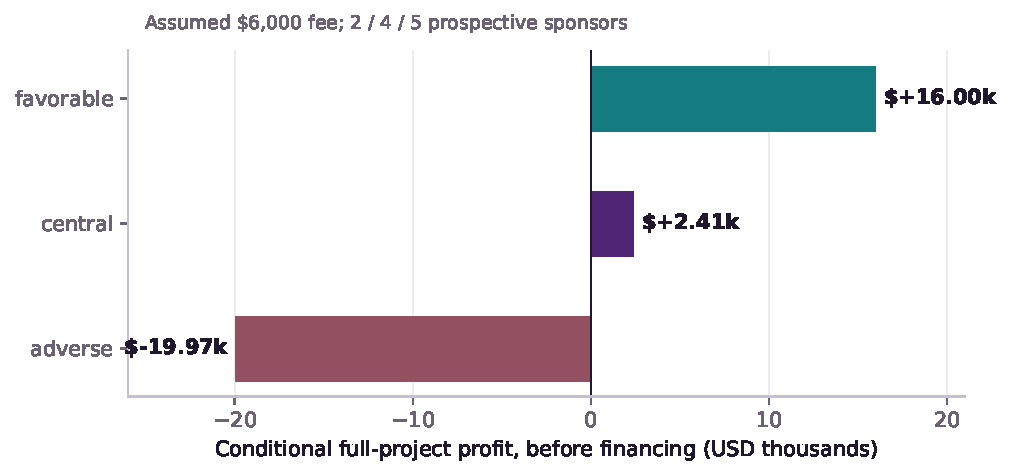
\includegraphics[width=0.95\textwidth,height=\textheight]{figures/economics.pdf}
\caption{Conditional full-project results. The central profit is modest
and depends on four paying sponsors; the adverse loss remains visible.
Actual revenue is zero and actual complete profit is unknown.}
\end{figure}

At four sponsors, the central break-even fee is USD5,379.38 each; at
USD6,000, four accepted payers are required. A fixed-assumption grid
varies one to twelve participants and eight fees. A
participation-sensitive schedule tests USD18,000 for one sponsor,
USD10,000 for two, USD6,000 for four, USD4,800 for six and USD4,000 for
eight. These conditional discounts reflect shared fixed costs; they are
neither a proven optimum nor evidence that participation rises at those
prices. An exclusivity requirement, incompatible integration environment
or unpaid sponsor changes the economics. A separate 60-case
value-pricing grid assumes a buyer value already net of internal costs
and incremental to the free public-artifact option, then tests capture
fractions of 25\%, 50\% and 75\%. At four buyers and 50\% capture, the
necessary net value for break-even is USD10,758.76 each. Hypothetical
value USD12,000 gives the USD6,000 central fee and USD2,408 project
profit; value USD6,000 gives a USD3,000 fee and USD9,232 loss. These are
required-value sensitivities, not measured buyer value or uptake. Fee
below value is only a necessary participation condition, not proof of
demand.

The cash model uses a refundable 40\% deposit, a 30\% payment at
accepted core delivery and 30\% at final acceptance. Deposits remain
restricted until earned. The central arrangement reaches an additional
unrestricted cash requirement of USD6,573.20 above the unchanged
USD5,000 capital. The plotted negative balance is a counterfactual stop
point: work cannot continue unfunded, and refundable deposits cannot
fill the gap.

\begin{figure}
\centering
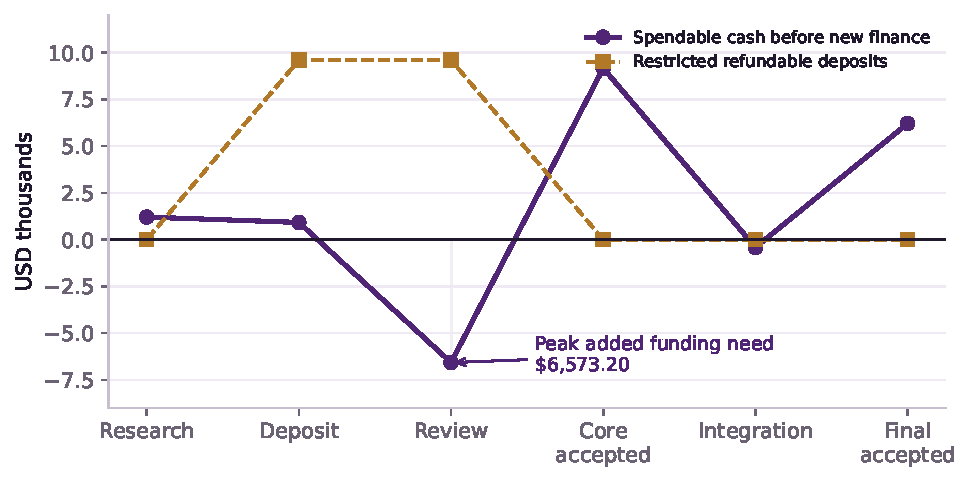
\includegraphics[width=0.95\textwidth,height=\textheight]{figures/cash.pdf}
\caption{Central cash timing before new finance. Refundable deposits
remain restricted. A positive project margin does not finance the review
work that precedes acceptance.}
\end{figure}

A hypothetical 90-day bridge at a 2\% origination charge and 12\% simple
annual interest requires USD6,707.35 principal to provide the needed net
proceeds. Its USD335.37 financing cost leaves conditional central profit
of USD2,072.63. This is a financing sensitivity, not an available lender
offer. Delayed acceptance, failed review or cancellation can make it
inadequate. Before first acceptance, cancellation returns the USD9,600
deposit and leaves USD11,573.20 unrecovered central cost.

Expected support and maintenance are already costed and assumed prepaid
at integration in the timing scenario. A remaining service obligation
survives final delivery. A separate reserve of 5\% of earned fees
encumbers cash for adverse obligations; it is not a second expense.
Financing principal, deposits, reserves, token issuance and token
appreciation are not operating earnings. All figures are pre-tax
planning values, with applicable pass-through taxes excluded from
revenue. Exact-rational accounting and a separately written cash
reconstruction agree.

\Needspace{7\baselineskip}

\hypertarget{complementarity-at-enterprise-level}{%
\subsection{Complementarity at enterprise
level}\label{complementarity-at-enterprise-level}}

The comparison includes the existing finite-search arrangement,
technical proof alone, coordination alone, both together, and an equally
capable conventional shared arrangement.

\begin{longtable}[]{@{}
  >{\raggedright\arraybackslash}p{(\columnwidth - 4\tabcolsep) * \real{0.3333}}
  >{\raggedright\arraybackslash}p{(\columnwidth - 4\tabcolsep) * \real{0.3333}}
  >{\raggedright\arraybackslash}p{(\columnwidth - 4\tabcolsep) * \real{0.3333}}@{}}
\toprule\noalign{}
\begin{minipage}[b]{\linewidth}\raggedright
Arrangement
\end{minipage} & \begin{minipage}[b]{\linewidth}\raggedright
Universal mathematical deliverable
\end{minipage} & \begin{minipage}[b]{\linewidth}\raggedright
Commercial interpretation
\end{minipage} \\
\midrule\noalign{}
\endhead
\bottomrule\noalign{}
\endlastfoot
Finite MILP alone & Not established & No sale credited for a universal
answer \\
New certificate; ordinary four-client delivery & Established digitally &
Conditional full-project profit of \$2,408 \\
Coordination of finite results & Not established & Shared payment does
not supply the missing proof \\
Certificate; four compatible sponsors & Established digitally &
Conditional full-project profit of \$2,408 \\
Conventional shared arrangement; same artifact & Same accepted result &
Same conditional \$2,408 profit \\
\end{longtable}

All accepted four-beneficiary arrangements hold buyer count, fees,
access, work and cost assumptions fixed. Ordinary acquisition and
coordination costs are included in each. They tie; no separate
incremental coordination benefit or exclusive technical-commercial
interaction is identified. A one-beneficiary case at the same assumed
USD6,000 fee loses USD10,774, but that is a participation sensitivity,
not a causal estimate that coordination creates three customers. The
supported conditional mechanism is sharing fixed review and publication
costs among compatible requirements. A numerical factorial interaction
is not estimated because the finite-search arms do not deliver the same
accepted product. Assigning them invented profitable sales would
manufacture a comparison.

Participants would need compatible acceptance terms, nonexclusive
access, clear rights to contributed code and an agreed allocation of
review, correction and withdrawal costs. No exclusive ownership of a
mathematical problem or theorem is sold. A sponsor can decline or use
the public artifact independently. These outside options make
willingness-to-pay validation essential. The arrangement would fail if
shared review is unacceptable, environments diverge, promised human
review cannot be staffed, or commitments do not become earned receipts.

\Needspace{9\baselineskip}

\hypertarget{a-successor-with-a-useful-inheritance}{%
\section{A successor with a useful
inheritance}\label{a-successor-with-a-useful-inheritance}}

\Needspace{7\baselineskip}

\hypertarget{retention-is-selective}{%
\subsection{Retention is selective}\label{retention-is-selective}}

The successor inherits both exact witnesses, their readable proofs,
independent checkers, scope rules, counterexamples and economic
boundaries. That is technical portability. It is not by itself net
Alpha.

Fresh scope tasks cover translated integer intervals, repeated moduli,
weaker thresholds and unsupported requests such as singletons, two
dimensions or a stronger bound. A competent recipient with the same
ordinary-library artifact has the same mathematical information. The
recorded scope decisions confirm supported reuse and refusal behavior
for their identified artifact; they are not an LLM performance
comparison. No incremental task benefit over that ordinary library was
measured.

Additional specialist packaging is modeled at USD1,042: USD330
extraction, USD280 extra validation, USD220 integration, USD200 upkeep
and USD12 storage. The planning model admits no unsupported incremental
benefit, so paid extraction is \textbf{HOLD}. Zero admitted benefit is
not a measured zero effect or a theorem that future benefit is
impossible. The existing research artifact remains useful without that
expenditure. Gym practice and further specialist training require a
fresh target and an economic reason; they are not automatic reinvestment
milestones.

\Needspace{7\baselineskip}

\hypertarget{frontier-model-operation-and-its-measurement-boundary}{%
\subsection{Frontier-model operation and its measurement
boundary}\label{frontier-model-operation-and-its-measurement-boundary}}

The live authoring session identifies GPT-6 Astra. Official
documentation inspected on the study date lists identifier
\texttt{gpt-6-astra}, a 1,050,000-token context window, a 128,000-token
output limit, tool use and configurable reasoning effort. Documented
standard short-context prices are USD10 per million input tokens, USD1
cached input and USD50 output; long-context and faster modes have
different rates (\protect\hyperlink{ref-openai2026model}{OpenAI 2026b},
\protect\hyperlink{ref-openai2026pricing}{2026a}). These are verified
planning references, not a bill for this session.

Work was decomposed into opportunity search, conventional challenge,
source/definition audit, construction, independent checking, economic
reconciliation and publication. Recovery included rejecting an
attractive infeasible polynomial and preserving corrected code. Those
are descriptions of expert operation. No local API credential, metered
provider call log, precise sampling configuration or complete
authoring-token bill was available. We therefore ran narrower executable
mathematical and accounting tests, not a simulated model-capability
measurement.

Operational Alpha would require a fresh, matched comparison of ordinary
and expert operation of the same model, with accepted outcomes, errors,
correction, human effort and resource cost all counted. This study does
not supply that comparison. Here the conventional challenger also
independently discovered a successful formulation for the selected
problem. That substantive success reinforces the absence of an exclusive
capability claim. A broader discovery comparison still needs matched
initial information, multiple fresh tasks and complete costs.

\Needspace{7\baselineskip}

\hypertarget{existing-ecosystem-components-actually-exercised}{%
\subsection{Existing ecosystem components, actually
exercised}\label{existing-ecosystem-components-actually-exercised}}

The study continues the inspected repository and issue history. It does
not replace the active execution, specialist or enterprise teams. The
native source closure contains 44 unchanged files pinned to commit
\texttt{47c17f6}, with byte equality checked against the inspected main
source. Separate native receipts bind the earlier polynomial artifact
and the final stronger certificate, including its corrected wrapper and
fresh confirmation hashes. An existing archive-study adapter is reused
unchanged (\protect\hyperlink{ref-coordination2026}{MONTREAL.AI 2026a},
\protect\hyperlink{ref-archive2026}{2026b}).

\textbf{Insight} produced a neutral single-candidate review dossier. It
records the selected result and checks its local structure; supplied
neutral scores do not measure opportunity discovery. \textbf{Nova-Seed}
records an unminted, unfunded research draft with provenance.
\textbf{FusionPlan} compiles and verifies four job commitments, with
altered-plan and altered-dossier refusals. A verified plan does not
assert that downstream jobs were executed. The existing production
capsule refuses the unsupported scientific scope.

The local Journal, Trust and CostLedger fixtures record four events and
reject a complete-cost seal while authoring costs are unknown. Profit
remains null. Temporary fixture identities are explicit identity
simulation, not live \texttt{*.agent.agi.eth} authentication. MARK
contracts and the review pathway were inspected, but MARK was not
activated. No minting, trading, spending, permission change, customer
contact or token operation occurred. USDC settlement and applicable
\$AGIALPHA utility remain distinct; neither contributes imaginary
revenue.

Cryptographic hashes protect the integrity of recorded content. They do
not establish scientific accuracy, ownership of an opportunity,
foresight or investment value. Publication is a research-review handoff
through the existing repository process, separate from a qualified
production release.

\Needspace{9\baselineskip}

\hypertarget{learning-from-the-existing-evidence}{%
\section{Learning from the existing
evidence}\label{learning-from-the-existing-evidence}}

Three foundations guide the study. \emph{Transformational Intelligence}
separates purpose, formulation and evaluation, and explicitly admits an
unrestricted optimal conventional planner. \emph{Invent the Economy}
distinguishes technical possibility, complete profitability and
financing; a positive project with insufficient prefunding differs from
one whose added costs make its profit negative. \emph{Transformational
Autonomous Enterprises} requires mission-specific revalidation and
comparison with a competent direct specialist, rather than counting
graph growth or imports as Alpha
(\protect\hyperlink{ref-transformational2026}{MONTREAL.AI 2026g},
\protect\hyperlink{ref-economy2026}{2026d},
\protect\hyperlink{ref-enterprises2026}{2026f}).

The recent event-history construction tied classical parity and closure.
The archive instrument made valid exact inferences but tied conventional
methods; its corrected economics and unresolved successor questions
prevented a flagship claim. The disclosure follow-up matched established
auditing and remained losing in its tested complete scenarios
(\protect\hyperlink{ref-event2026}{MONTREAL.AI 2026c},
\protect\hyperlink{ref-archive2026}{2026b},
\protect\hyperlink{ref-disclosure2026}{2026e}). These are different
offerings; their profits and losses are not imported into this study.

The requested DNA-encoding lesson is retained as user-supplied prior
context: a useful construction was matched conventionally. Targeted
source and file searches did not resolve its exact artifact. We
therefore do not invent its case counts, financial figures or a source
path. This unresolved lineage item does not support a positive claim
here.

The practical correction is earlier challenge. Broad mechanisms already
supplied by prior art were stopped before implementation. Known code
records were preserved as strong baselines. The infeasible polynomial
was rejected despite its attractive numerical integral. The final paper
leads with the checked theorem while keeping commercial and comparative
limits beside it.

\Needspace{9\baselineskip}

\hypertarget{three-horizons-with-explicit-dependencies}{%
\section{Three horizons, with explicit
dependencies}\label{three-horizons-with-explicit-dependencies}}

\textbf{Near term --- a durable mathematical result.} The completed
capability is a locally reproducible, exact answer to the stated
covering question, with two implementations, fresh checks, a refusal
boundary and a retained failure history. Its scientific significance is
a stronger universal bound and a reusable proof artifact. Its actual
commercial return is unmeasured. External expert review of definitions,
mathematics and priority is the smallest decisive next scientific step.

\textbf{Expansion --- a portfolio of accepted certificates.} Related
finite-cover parameters, sharper constants and other discrete
construction problems are plausible fresh work. Each needs a fixed
externally meaningful target, unrestricted conventional search, a proof
or independently accepted witness, full costs and a refusal if the
target is missed. A certificate-review service additionally needs a real
sponsor's acceptance criteria, resource quote, willingness to pay and
financing commitment. Failure of external review, conventional
equivalence without separately demonstrated discovery value, or
insufficient paid demand falsifies the respective expansion claim.

\textbf{Long term --- productive infrastructure for discovery.} The
ambition is an enterprise that builds instruments, representations and
evidence others can use to undertake work previously unsupported by
their available artifacts. A reliable portfolio could support new
research collaborations; validated delivery and transferable capability
could support broader instruments. Repeated useful discoveries,
independent acceptance, economic surplus and selective retention are
separate causal steps. None implies inevitable acceleration, a measured
enterprise valuation or ownership of a future industry.

The successor receives something concrete: a problem boundary it no
longer needs to guess, the means to verify that boundary, and an honest
record of where the result stops. \textbf{Find your Alpha. Build your
SUCCESSOR \(\Omega\).}

\clearpage

\Needspace{9\baselineskip}

\hypertarget{appendix-a.-a-universal-piecewise-linear-weight-certificate}{%
\section{Appendix A. A universal piecewise-linear weight
certificate}\label{appendix-a.-a-universal-piecewise-linear-weight-certificate}}

\Needspace{7\baselineskip}

\hypertarget{a.1-statement-and-exact-coefficients}{%
\subsection{A.1 Statement and exact
coefficients}\label{a.1-statement-and-exact-coefficients}}

\begin{samepage}

Let finitely many complete residue classes, restricted to the integers
\(1,\ldots,n\), partition that interval. Suppose each restriction
contains at least two integers. If their moduli are \(m_1,\ldots,m_r\),
then

\[
\boxed{\displaystyle h=\sum_{i=1}^r\frac1{m_i}
\ge J:=\frac{17902560}{18258529}
=0.9805039606421744\ldots>\frac{49}{50}.}
\]

\end{samepage}

The proof permits repeated moduli and therefore answers the original
distinct-modulus question. It retains complete restrictions, exact
partitioning and the minimum of two interval elements per class. No
optimality assertion accompanies the constant \(J\).

Define \(W\) as the continuous linear interpolant at the knots \(j/20\),
for \(0\le j\le20\), with \(W(1-x)=W(x)\) and the following integer
coefficients. Extend \(W\) by zero outside \([0,1]\).

\begin{longtable}[]{@{}rr@{}}
\toprule\noalign{}
\(j\) & \(W(j/20)\) \\
\midrule\noalign{}
\endhead
\bottomrule\noalign{}
\endlastfoot
0 & 0 \\
1 & 159 \\
2 & 316 \\
3 & 493 \\
4 & 721 \\
5 & 981 \\
6 & 1240 \\
7 & 1500 \\
8 & 1658 \\
9 & 1818 \\
10 & 1858 \\
\end{longtable}

\begin{samepage}

Reflection supplies the remaining ten coefficients. Exact trapezoid
integration and summation of derivative jumps give

\[
I_W:=\int_0^1W(x)\,dx=\frac{1963}{2},
\qquad V:=\operatorname{TV}(W')=21200.
\]

\end{samepage}

\begin{samepage}

Here \(W'\) denotes the derivative of the zero extension. Its variation
includes the jumps from zero derivative at both support endpoints. The
normalization used below is

\[M=\frac{18258529}{18240},\qquad J=\frac{I_W}{M}.\]

\end{samepage}

\Needspace{7\baselineskip}

\hypertarget{a.2-the-complete-progression-domain}{%
\subsection{A.2 The complete progression
domain}\label{a.2-the-complete-progression-domain}}

\begin{samepage}

For \(k\ge2\), consider the sum

\[S_k(a,d)=d\sum_{\ell=0}^{k-1}W(a+\ell d),\qquad d>0.\]

\end{samepage}

\begin{samepage}

The closed domain

\[
D_k=\{(a,d):0\le a\le d,\quad a+(k-1)d\le1\le a+kd\}
\]

\end{samepage}

\begin{samepage}

contains every complete \(k\)-point progression in the open unit
interval. The inequalities allow its predecessor or successor to lie at
an endpoint; this enlargement is harmless because \(W(0)=W(1)=0\). In
particular,

\[\frac1{k+1}\le d\le\frac1{k-1}.\]

\end{samepage}

\begin{samepage}

The domain is the compact quadrilateral with consecutive vertices

\[
\left(\frac1{k+1},\frac1{k+1}\right),\quad
\left(\frac1k,\frac1k\right),\quad
\left(0,\frac1{k-1}\right),\quad
\left(0,\frac1k\right).
\]

\end{samepage}

We prove \(S_k\le M\) throughout \(D_k\) for every \(k\ge2\).

\Needspace{7\baselineskip}

\hypertarget{a.3-exact-maximization-for-short-progressions}{%
\subsection{A.3 Exact maximization for short
progressions}\label{a.3-exact-maximization-for-short-progressions}}

\begin{samepage}

For each \(2\le k\le20\), subdivide \(D_k\) by all knot-crossing lines

\[a+jd=\frac r{20},\qquad 0\le j<k,\quad 0\le r\le20.\]

\end{samepage}

\begin{samepage}

On each resulting polygonal cell, the arguments of \(W\) stay in fixed
linear pieces. Consequently

\[S_k(a,d)=Aad+Bd^2+Cd\]

\end{samepage}

for constant rational coefficients. If \(A\ne0\), its Hessian has
determinant \(-A^2<0\), excluding an interior local maximum.
Equivalently, its derivative in \(a\) is the nonzero quantity \(Ad\). If
\(A=0\), the objective is independent of \(a\): a maximizing section at
fixed \(d\) reaches the cell boundary with the same value. Degenerate
cells already belong to boundaries. Thus a global maximum occurs on an
enumerated boundary, including possible stationary ridges.

Every boundary is a knot-crossing line or one of the four edges of
\(D_k\). The lines with \((j,r)=(0,0)\) and \((k-1,20)\) cover \(a=0\)
and \(a+(k-1)d=1\). The remaining edges are included explicitly as
\((j,r)=(-1,0)\) and \((k,20)\), representing \(a=d\) and \(a+kd=1\).

\begin{samepage}

On a fixed line \(a+jd=r/20\), every crossing with another knot line
occurs at

\[d=\frac{s-r}{20(\ell-j)},\qquad \ell\ne j.\]

\end{samepage}

The domain endpoints and these crossings divide the line into finitely
many rational segments. On each, \(S_k=\alpha d^2+\beta d\). Its maximum
occurs at an endpoint or, when \(\alpha<0\), at the stationary point
\(-\beta/(2\alpha)\) if that point belongs to the segment. Degenerate
point segments are also evaluated.

\begin{samepage}

The standard-library checker
\texttt{fresh\_conventional/verify\_weight.py} implements this
enumeration using exact integers and fractions. All nineteen
cardinalities pass, and their largest value is precisely

\[M=\frac{18258529}{18240},\]

\end{samepage}

attained at \(k=2\), \(a=7/20\) and \(d=4273/9120\). The original
enumeration checks 1,967 segments, including point cases and repeated
descriptions.

The independent checker \texttt{lineage/audit\_conventional\_weight.py}
reconstructs line segments by intersecting polygon edges, rather than by
the first checker's inequality-clipping formulas. It interpolates \(W\)
directly, reconstructs each quadratic from exact endpoint values, checks
its midpoint identity and evaluates stationary points directly. It
reproduces every per-cardinality maximum. Its different bookkeeping
gives 1,863 positive-length segments and 360 interior stationary
evaluations, with degenerate points checked separately. The audit
receipt is
\texttt{confirmation/conventional\_independent/INDEPENDENT\_WEIGHT\_AUDIT.json}.
These are separate implementations within one study, not external peer
review or proof-assistant verification.

\Needspace{7\baselineskip}

\hypertarget{a.4-an-analytic-bound-for-all-remaining-cardinalities}{%
\subsection{A.4 An analytic bound for all remaining
cardinalities}\label{a.4-an-analytic-bound-for-all-remaining-cardinalities}}

\begin{samepage}

For a continuous compactly supported piecewise-linear function, the
composite trapezoid estimate on a lattice of spacing \(d\) is

\[
\left|d\sum_{z\in\mathbb Z}W(a+zd)-\int_{\mathbb R}W(x)\,dx\right|
\le\frac{d^2}{8}\operatorname{TV}(W').
\]

\end{samepage}

Indeed, on a lattice cell \([u,u+d]\), the trapezoid error is the
integral of \((x-u)(u+d-x)/2\) against the signed measure of derivative
jumps. This kernel has magnitude at most \(d^2/8\). Summing over cells
and using the measure's total variation proves the estimate. Endpoint
jumps of the zero extension are included, so cells crossing the support
boundary require no exception.

\begin{samepage}

For \((a,d)\in D_k\), the listed progression contains every nonzero
contribution of the lattice. When \(k\ge21\), the bound \(d\le1/20\)
therefore gives

\[
S_k(a,d)\le\frac{1963}{2}+\frac{21200}{8\cdot20^2}
=\frac{7905}{8}<M.
\]

\end{samepage}

Together with the finite exact computation, this proves \(S_k\le M\) for
every admissible progression, without a cardinality cutoff.

\Needspace{7\baselineskip}

\hypertarget{a.5-exact-transfer-to-every-integer-interval}{%
\subsection{A.5 Exact transfer to every integer
interval}\label{a.5-exact-transfer-to-every-integer-interval}}

\begin{samepage}

For an arbitrary partition of \(\{1,\ldots,n\}\), define cell-integral
weights

\[w_j=\int_{(j-1)/n}^{j/n}W(x)\,dx.\]

\end{samepage}

\begin{samepage}

Consider a complete restricted residue class \(C\) modulo \(m\). For
each \(0<t<1\), its points

\[x_j(t)=\frac{j-1+t}{n},\qquad j\in C,\]

\end{samepage}

form a progression of spacing \(d=m/n\) with at least two members. Its
predecessor integer is at most zero, so its normalized predecessor is at
most \((-1+t)/n<0\). Its successor integer is at least \(n+1\), so its
normalized successor is at least \(1+t/n>1\). The progression thus
belongs to \(D_{|C|}\).

\begin{samepage}

Integrating its certified inequality in \(t\) yields

\[
\frac mn\sum_{j\in C}\int_0^1W\!\left(\frac{j-1+t}{n}\right)dt
=m\sum_{j\in C}w_j\le M.
\]

\end{samepage}

Sum over the partition. Every integer cell occurs once, giving
\(I_W\le Mh\) and hence \(h\ge J\). This applies directly to every
admissible \(n\); no limiting argument, midpoint correction or
unverified small-length case remains. For \(n=1\) the hypotheses are
impossible.

\Needspace{7\baselineskip}

\hypertarget{a.6-normalization-and-contribution}{%
\subsection{A.6 Normalization and
contribution}\label{a.6-normalization-and-contribution}}

The discovery report used the convenient safe scale \(T=2003/2\),
obtaining \(h\ge1963/2003>0.98\). Its computation already established
the smaller exact maximum \(M\). Normalizing by \(M\) gives the stronger
bound \(J\) without changing the knots, domain or proof obligations. The
theorem states \(h\ge J\); it does not assert strictness at \(J\).

Discovery used standard linear and mixed-integer optimization, followed
by exact rational geometry and a classical quadrature estimate. The
contribution is the explicit certificate and resulting universal bound.
It establishes neither a new general solver nor an exclusive AI
capability or controlled discovery advantage.

\Needspace{9\baselineskip}

\hypertarget{appendix-b.-the-earlier-polynomial-proof}{%
\section{Appendix B. The earlier polynomial
proof}\label{appendix-b.-the-earlier-polynomial-proof}}

\Needspace{7\baselineskip}

\hypertarget{b.1-definition-and-exact-witness}{%
\subsection{B.1 Definition and exact
witness}\label{b.1-definition-and-exact-witness}}

Let a complete residue class modulo a positive integer \(m\) be
restricted to \(\{1,\ldots,n\}\). Suppose finitely many such
restrictions partition that interval and each contains at least two
points. Repeated moduli are allowed in this proof. Let \(h\) be the sum
of reciprocal moduli.

\begin{samepage}

The coefficient vector, in increasing even Chebyshev order, is

\[
\begin{aligned}
(b_0,\ldots,b_{10})={}&(7061527976,-8616261687,2079655784,\\
&-480883959,30533879,8370806,32646497,\\
&-16295510,3707761,-15109523,30943868).
\end{aligned}
\]

\end{samepage}

\begin{samepage}

Let \(T_r\) denote the Chebyshev polynomial of the first kind. Define

\[f(x)=\frac{2499}{2500\cdot10^{10}}\sum_{j=0}^{10} b_jT_{2j}(2x-1).\]

\end{samepage}

\begin{samepage}

It satisfies \(f(1-x)=f(x)\). Each basis element has integral
\((1-4j^2)^{-1}\) on \([0,1]\), so the exact witness integral is

\[I=\frac{1891871140656049}{1929687500000000}=0.9804028583156853\ldots.\]

\end{samepage}

\Needspace{7\baselineskip}

\hypertarget{b.2-the-class-domain-and-the-dual-argument}{%
\subsection{B.2 The class domain and the dual
argument}\label{b.2-the-class-domain-and-the-dual-argument}}

\begin{samepage}

A class has interval hits \(r,r+m,\ldots,r+(k-1)m\), where \(k\ge2\).
Put \(d=m/n\) and \(a=(r-1/2)/n\). The previous and next members lie
outside the interval. Consequently

\[
\max(0,1-kd)\le a\le\min(d,1-(k-1)d),
\qquad \frac1{k+1}\le d\le\frac1{k-1}.
\]

\end{samepage}

\begin{samepage}

These closed inequalities relax the strict exterior conditions of actual
integer classes and thus enlarge the checked domain. Define the class
constraint

\[d\sum_{j=0}^{k-1}f(a+jd)\le1.\tag{B1}\]

\end{samepage}

\begin{samepage}

Assign integer \(i\) the weight \(f((i-1/2)/n)/n\). If (B1) holds, the
class's assigned weight is at most \(1/m\). Exact partitioning then
yields

\[h\ge M_n:=\frac1n\sum_{r=1}^n f((r-1/2)/n).\tag{B2}\]

\end{samepage}

There is no sign restriction on individual weights in this summation
argument. We next establish (B1) for every class and \(M_n>I\) for every
\(n\ge2\).

\Needspace{7\baselineskip}

\hypertarget{b.3-every-short-class-78-exact-continuous-certificates}{%
\subsection{B.3 Every short class: 78 exact continuous
certificates}\label{b.3-every-short-class-78-exact-continuous-certificates}}

\begin{samepage}

Write \(F(z)=f((z+1)/2)\) and \(u=2a+(k-1)d-1\). Reflection of the class
allows \(u\ge0\) because \(F\) is even. The admissible domain becomes

\[0\le u\le\min((k+1)d-1,1-(k-1)d).\]

\end{samepage}

\begin{samepage}

For \((s,v)\in[0,1]^2\), its two halves are parameterized by

\[
\begin{array}{lll}
\text{lower spacing:}&d=(k+s)/(k(k+1)),&u=vs/k,\\
\text{upper spacing:}&d=(k-1+s)/(k(k-1)),&u=v(1-s)/k.
\end{array}
\]

\end{samepage}

\begin{samepage}

For each \(k=2,\ldots,40\) and each half, the polynomial

\[P_k(s,v)=1-d\sum_{j=0}^{k-1}F\big(u+(2j-k+1)d\big)\]

\end{samepage}

has bidegree at most \((21,20)\). Clear its positive rational
denominator and transform to the tensor Bernstein basis. A polynomial in
that basis is a convex combination of its coefficients on the unit
square. Nonnegative coefficients therefore prove \(P_k\ge0\) on that
square. Exact de Casteljau midpoint subdivision applies the same test on
smaller rectangles whose union is the original square.

\begin{samepage}

The primary checker uses the identity

\[
\sum_{j=0}^{k-1}(u+(2j-k+1)d)^\ell
=\sum_{r=0}^{\ell}{\ell\choose r}u^{\ell-r}d^r
\sum_{j=0}^{k-1}(2j-k+1)^r.
\]

\end{samepage}

Symmetry eliminates the odd terms. After clearing the coefficient
denominator, a common denominator contains \([k(k\pm1)]^{21}\) and is
positive. All 78 patches pass: 106 visited nodes, 92 accepted leaves and
maximum subdivision depth six. The independent sparse-Horner
implementation checks the same polynomials with a different conversion
and subdivision sequence: 95 accepted leaves and the same maximum depth.
Exact leaf rectangles and bounds are retained. Different trees do not
change the covered domain.

\Needspace{7\baselineskip}

\hypertarget{b.4-every-larger-class-an-analytic-tail}{%
\subsection{B.4 Every larger class: an analytic
tail}\label{b.4-every-larger-class-an-analytic-tail}}

\begin{samepage}

Define \(g=f-f(0)\) on \([0,1]\) and extend it by zero to the real line.
Symmetry makes this extension continuous. Exact univariate Bernstein
bounds on 64 rational subintervals give

\[|f(0)|<3/250,\qquad \|f''\|_\infty<486,
\qquad \operatorname{TV}(g')<24.\]

\end{samepage}

The variation includes both endpoint jumps of the extended derivative.
Its tighter computed upper bound is approximately 23.05544856893; the
second-derivative bound is approximately 485.76248165584. Both arise
from rational inequalities, not rounded acceptance thresholds.

\begin{samepage}

For a continuous compactly supported function whose derivative has
bounded variation, the shifted-grid trapezoid bound is

\[
\left|d\sum_{j\in\mathbb Z}g(a+jd)-\int_{\mathbb R}g(x)\,dx\right|
\le\frac{d^2}{8}\operatorname{TV}(g').
\]

\end{samepage}

To obtain the constant, integrate the piecewise-linear interpolation
error on each grid cell against the distributional second derivative.
The corresponding kernel has magnitude at most \(d^2/8\); summing the
variation over cells gives the bound. The integral of the interpolant
equals the composite trapezoid sum. Zero extension and continuity
account for cells crossing the endpoints.

\begin{samepage}

For a complete class, \(|kd-1|\le d\). Adding back \(f(0)\) gives

\[
d\sum_{j=0}^{k-1}f(a+jd)
\le I+|f(0)|d+\frac{d^2}{8}\operatorname{TV}(g').
\]

\end{samepage}

\begin{samepage}

For \(k\ge41\), \(d\le1/40\), so the right side is at most

\[I+\frac3{10000}+\frac3{1600}=I+0.002175<1.\]

\end{samepage}

Thus (B1) holds for every larger class as well. The independent tighter
rational bound is approximately 0.98250103613, also strictly below one.

\Needspace{7\baselineskip}

\hypertarget{b.5-every-interval-length-the-strict-objective}{%
\subsection{B.5 Every interval length: the strict
objective}\label{b.5-every-interval-length-the-strict-objective}}

\begin{samepage}

Let \(t=1/n^2\), \(z_i=(2i-1-n)/n\) and
\(A_r(t)=n^{-1}\sum_i z_i^{2r}\). The identity

\[\sum_{i=1}^n\big((z_i+1/n)^{2r+1}-(z_i-1/n)^{2r+1}\big)=2\]

\end{samepage}

\begin{samepage}

telescopes. Binomial expansion gives

\[
A_0(t)=1,\qquad
A_r(t)=\frac{1-\sum_{\ell=1}^{r}{2r+1\choose2\ell+1}t^\ell A_{r-\ell}(t)}{2r+1}.
\]

\end{samepage}

\begin{samepage}

Writing \(F(z)=\sum_{r=0}^{10}c_rz^{2r}\), this yields the exact
identity

\[M_n=\sum_{r=0}^{10}c_rA_r(t)=I+tQ(t),\]

\end{samepage}

where \(Q\) has degree nine. The coefficient list agrees exactly with a
separate Euler--Maclaurin derivation. The independent checker uses an
explicit Chebyshev coefficient formula and the telescoping recurrence,
without importing the first derivation.

\begin{samepage}

All Bernstein coefficients of \(Q\) are strictly positive on each of the
16 intervals \([j/256,(j+1)/256]\), \(j=0,\ldots,15\). Hence \(Q(t)>0\)
on \([0,1/16]\), which covers every \(n\ge4\). The two remaining exact
differences are

\[M_2-I=\frac{184569613348897}{61750000000000000}>0,\]

\end{samepage}

\begin{samepage}

\[M_3-I=\frac{1033236506971259179273363}{53827234190437500000000000}>0.\]

\end{samepage}

Therefore \(M_n>I\) for every \(n\ge2\). Together with (B2), this proves
\(h>I\). The JSON evidence contains every rational coefficient and each
positive interval bound.

A redundant weaker completion also survives: the midpoint-remainder
inequality gives \(M_n>I-486/(24n^2)>0.98\) for \(n\ge225\), with
smaller \(n\) checked exactly. This overlap provides an additional check
on the original threshold conclusion; it is not needed for the stronger
constant.

\Needspace{9\baselineskip}

\hypertarget{appendix-c.-study-protocol-failures-and-comparison-limits}{%
\section{Appendix C. Study protocol, failures and comparison
limits}\label{appendix-c.-study-protocol-failures-and-comparison-limits}}

\Needspace{7\baselineskip}

\hypertarget{c.1-budget-and-chronology}{%
\subsection{C.1 Budget and chronology}\label{c.1-budget-and-chronology}}

The initial protocol was recorded with start time 21:57:28 UTC on 27
October 2026, a 120-minute wall ceiling, at most four concurrent
workers, a 30 CPU-minute deliberate-search ceiling and a 1,300 MiB
memory ceiling per search. It reserved at least 35 minutes for fresh
confirmation, reconciliation and publication. No external spending was
authorized or performed. Search, source inspection and publication are
different resource categories. Complete aggregate CPU and peak-memory
telemetry were not captured; the package records per-run limits and
available elapsed/CPU observations rather than certifying an exact
total. Complete model billing remains unavailable.

The first checkpoint was the diverse opportunity screen and strongest
identified conventional challenges. The second was the working exact
certificate and provisional decision. The polynomial witness and checker
files were frozen for confirmation at 22:21:02 UTC. After the stronger
conventional result passed independent audit, a separate final freeze
was recorded at 22:30:41 UTC. An independent malformed-request check
then found a JSON-null interface error; the corrected final wrapper
received an additive second freeze before its final adverse suite. All
snapshots are preserved. The supplemental exact-case plan was recorded
before those fresh cases were executed. Numerical search configuration
was consolidated after discovery and is explicitly retrospective; it is
not presented as preregistration.

Early stop rules included a same-requirement conventional match, no
independently checked improvement, resource exhaustion and unavailable
authorized access. The zero-error lane was stopped without a record
claim. The initial polynomial was rejected. The final mathematical claim
survives the exact checks, while commercial validation, exclusive
capability and discovery Alpha remain unestablished. Publication is
bounded to this review edition; no continuous indefinite search is
implied.

\Needspace{7\baselineskip}

\hypertarget{c.2-preserved-conventional-results}{%
\subsection{C.2 Preserved conventional
results}\label{c.2-preserved-conventional-results}}

The \(C_{15}^3\) code baseline contains 383 words, verified
independently against all 73,153 word pairs and 3,064 permitted channel
outputs. A 30-second unseeded global MILP found only 338, so it was
never substituted for the stronger baseline. Two approximately
180-second seeded neighborhood searches retained 383. These are bounded
search outcomes, not optimality or impossibility proofs.

The \(C_7^5\) reconfiguration search exhausted 243 states within its
one-exchange class without finding a 368th word. Product/switch searches
reproduced 134,753 words in \(C_7^{10}\) but did not improve the known
construction. Subsequent primary-source inspection found stronger
asymptotic recursion results, so older July bounds were not used as the
final asymptotic comparator (\protect\hyperlink{ref-itty2026}{Itty et
al. 2026}; \protect\hyperlink{ref-buys2026}{Buys, Polak, and Zuiddam
2026}; \protect\hyperlink{ref-tandon2026}{Tandon 2026}). No
physical-channel claim or market price is derived from these
mathematical reproductions.

\Needspace{7\baselineskip}

\hypertarget{c.3-correction-and-refusal-inventory}{%
\subsection{C.3 Correction and refusal
inventory}\label{c.3-correction-and-refusal-inventory}}

The package preserves the infeasible coarse-grid polynomial, its
continuous and exact finite counterexamples, eight numerical refinement
iterations, finite-cover incumbents, failed and corrected all-length
code, the independent proof receipts and malformed-input controls.
Original archived outputs are not overwritten by the public reproduction
command.

The wrapper refuses a stronger requested bound, a two-dimensional
request, singleton classes, arbitrary selected progressions, non-exact
coverage, malformed rational input, altered witness bytes, changed
checker source, missing inputs, optimized Python and reuse of an
existing output directory. An admitted request establishes only the
theorem's conditional conclusion. It never asserts that a covering
system with the supplied extra properties exists.

\Needspace{7\baselineskip}

\hypertarget{c.4-what-independent-means-here}{%
\subsection{C.4 What ``independent'' means
here}\label{c.4-what-independent-means-here}}

Parallel workstreams share a model family and one coordinated study.
They are not independent human laboratories. Separation of code,
derivations, inputs and review roles reduces some correlated-error
risks; it does not eliminate them. The fresh conventional workstream
began without access to the selected witness. The source audit checked
original definitions and a stronger prior bound, preventing an
exaggerated comparison. External qualified review remains necessary
before treating this research-review edition as a settled canonical
reference.

\Needspace{9\baselineskip}

\hypertarget{appendix-d.-economic-assumptions-and-reconciliation}{%
\section{Appendix D. Economic assumptions and
reconciliation}\label{appendix-d.-economic-assumptions-and-reconciliation}}

All money is USD. Hours and rates below are analyst resource estimates,
not observed labor or market quotations. The fixed activities sum to 110
hours; marginal activities sum to 10.5 hours per beneficiary.

\begin{longtable}[]{@{}lrr@{}}
\toprule\noalign{}
Fixed activity & Hours & Assumed hourly rate \\
\midrule\noalign{}
\endhead
\bottomrule\noalign{}
\endlastfoot
Discovery, including failed searches & 24 & \$110 \\
Certificate construction and repair & 18 & \$110 \\
Independent mathematical review & 20 & \$140 \\
Publication and reproduction & 12 & \$90 \\
Correction and failed-review allowance & 12 & \$110 \\
Oversight, rights and commitments & 6 & \$120 \\
Acquisition and coordination & 10 & \$100 \\
One-year shared maintenance & 8 & \$100 \\
\end{longtable}

\begin{longtable}[]{@{}lrr@{}}
\toprule\noalign{}
Per-beneficiary activity & Hours & Assumed hourly rate \\
\midrule\noalign{}
\endhead
\bottomrule\noalign{}
\endlastfoot
Integration & 4 & \$110 \\
Acceptance and independent reproduction & 2 & \$140 \\
Onboarding & 1 & \$90 \\
Support & 2 & \$90 \\
Correction and failure allowance & 1.5 & \$110 \\
\end{longtable}

Add 20\% labor overhead; fixed USD300 research/verification compute and
USD60 storage/distribution; and USD40 per beneficiary. General
administration, tools, insurance and unallocated support are in overhead
and are not charged again. Processing is 3\% of fees. Discovery and
construction, including compute, contribute USD5,844 once to the central
project cost. All expected maintenance and correction are included
before profit is computed.

Central gross end cash before financing equals initial USD5,000 plus
full-project profit USD2,408. USD1,200 is encumbered by the additional
warranty reserve. That reserve does not remove the remaining service
duty. The six-stage ledger separately reports gross cash, restricted
refundable deposits, earned revenue, paid or prepaid costs, modeled cost
to complete, support prepayment and spendable cash. Infeasible
unfinanced balances are labeled as projections that require stopping,
not as executed spending.

At the assumed USD6,000 fee, an additional paying sponsor contributes
USD4,394 before fixed costs, provided requirements and marginal workload
remain unchanged. At four sponsors, a USD1,000 increase in the shared
cost reduces project profit by USD1,000; a USD1,000 fee decrease per
sponsor reduces profit by USD3,880 after the 3\% fee. These
sensitivities show why a modest positive central margin is not robust
evidence of a business.

The executable model emits complete scenario, activity, cash,
participation/fee, discount and arrangement tables. Its own audit
executes 153 exact accounting assertions. A separately written
implementation reconstructs all three scenarios and their cash ledgers
without importing the model. No scenario includes future token gains,
speculative enterprise valuation or profits copied from predecessor
studies.

\Needspace{9\baselineskip}

\hypertarget{appendix-e.-reproduction-evidence-and-publication-status}{%
\section{Appendix E. Reproduction, evidence and publication
status}\label{appendix-e.-reproduction-evidence-and-publication-status}}

\Needspace{7\baselineskip}

\hypertarget{e.1-minimal-exact-reproduction}{%
\subsection{E.1 Minimal exact
reproduction}\label{e.1-minimal-exact-reproduction}}

Python 3.11--3.13 with its standard library suffices for the fixed
mathematical certificate. From the package root, run:

\begin{Shaded}
\begin{Highlighting}[]
\ExtensionTok{python}\NormalTok{ final\_certificate.py }\DataTypeTok{\textbackslash{}}
  \AttributeTok{{-}{-}request}\NormalTok{ study/final\_request.json }\DataTypeTok{\textbackslash{}}
  \AttributeTok{{-}{-}output}\NormalTok{ local\_reproduction}
\end{Highlighting}
\end{Shaded}

The output directory must be new. The command copies the frozen checkers
into a temporary work area, recomputes both line-arrangement verifiers,
their exact maximum and the tail bound, checks complete obligation
coverage, and writes a new acceptance receipt. It does not rely on
stored success flags alone. \texttt{python\ reproduce.py} additionally
runs accounting reconciliation and package checks. Native ecosystem
execution is optional because its unchanged dependency closure requires
the documented packages.

Re-running floating-point discovery requires NumPy 2.3.2 and SciPy
1.17.0 in the recorded environment. Optimizer time limits can change
incumbents across machines. The reproducible theorem is the exact
rational certificate and its verification, not deterministic rediscovery
by a language model. Seeds, search limits, library versions and original
outputs are preserved.

\Needspace{7\baselineskip}

\hypertarget{e.2-claim-to-evidence-discipline}{%
\subsection{E.2 Claim-to-evidence
discipline}\label{e.2-claim-to-evidence-discipline}}

The evidence map labels claims as \textbf{executed}, \textbf{measured},
\textbf{independently checked}, \textbf{modeled}, \textbf{inferred} or
\textbf{proposed}. Mathematical validity rests on the explicit proof and
computational obligations. Wall-time values are local measurements.
Priority is a bounded inference from inspected primary sources.
Commercial fees and costs are modeled. Future services and broader
infrastructure are proposed. No simulated frontier-model capability is
reported.

Important files include \texttt{certificate/weight.json},
\texttt{final\_certificate.py}, both line-arrangement checkers,
\texttt{study/final\_confirmation\_protocol.json}, the earlier
polynomial sources and frozen protocol, fresh confirmation receipts, the
native integration manifest, \texttt{economics/results.json}, the
separate cash replay, \texttt{evidence/claim\_to\_evidence.csv} and
\texttt{evidence/prior\_art.csv}. The earlier polynomial witness SHA-256
begins \texttt{c92bc1977bbb6804}; the final witness and all source
hashes are recorded separately in the final freeze and package manifest.
Full copyrighted research working copies are excluded; citations and
authored audits remain.

\Needspace{7\baselineskip}

\hypertarget{e.3-review-edition-and-canonical-release}{%
\subsection{E.3 Review edition and canonical
release}\label{e.3-review-edition-and-canonical-release}}

This is a pinned research-review edition with a complete downloadable
package and a browser-readable counterpart generated from the same
manuscript. It is distinct from a merged canonical release, production
host qualification, external peer review or customer acceptance.
Repository publication must preserve existing originals and use a new
edition ID. Canonical catalog promotion follows the existing paper
importer and normal review/check process; executable additions retain
the applicable source acceptance gates.

The repository's main source was initially inspected at
\texttt{def7cdfc}; a later refresh found \texttt{3947e4ec}, the merge of
the existing 1.46.1 test-edition repair. This study uses a new directory
and does not take over that release owner or rewrite prior studies.
Public review URLs and immutable commit identity are recorded in the
separate publication receipt after verification. The LinkedIn text is an
approval draft and has not been posted.

\textbf{AI assistance and review disclosure.} The requested author line
is retained. GPT-6 Astra and parallel AI workstreams assisted source
review, mathematics, code, auditing and writing. Internal cross-checks
are described explicitly; no human peer review, model training, live ENS
identity, paid sponsor commitment or complete billing evidence is
implied.

\Needspace{9\baselineskip}

\hypertarget{references}{%
\section{References}\label{references}}

\hypertarget{refs}{}
\begin{CSLReferences}{1}{0}
\leavevmode\vadjust pre{\hypertarget{ref-bloem2015}{}}%
Bloem, Roderick, Bettina Könighofer, Robert Könighofer, and Chao Wang.
2015. {``Shield Synthesis: Runtime Enforcement for Reactive Systems.''}
\url{https://arxiv.org/abs/1501.02573}.

\leavevmode\vadjust pre{\hypertarget{ref-buys2026}{}}%
Buys, Pjotr, Sven Polak, and Jeroen Zuiddam. 2026. {``Lean-Verified
Lower Bounds for the Shannon Capacity of Odd Cycles.''}
\url{https://arxiv.org/abs/2607.29681}.

\leavevmode\vadjust pre{\hypertarget{ref-crisostomi2024}{}}%
Crisostomi, Donato, Marco Fumero, Daniele Baieri, Florian Bernard, and
Emanuele Rodolà. 2024. {``{C2M3}: Cycle-Consistent Multi-Model
Merging.''} In \emph{Advances in Neural Information Processing Systems}.
Vol. 37. \url{https://doi.org/10.52202/079017-0901}.

\leavevmode\vadjust pre{\hypertarget{ref-duarte2024}{}}%
Duarte, Guilherme, Noam Finkelstein, Dean Knox, Jonathan Mummolo, and
Ilya Shpitser. 2024. {``An Automated Approach to Causal Inference in
Discrete Settings.''} \emph{Journal of the American Statistical
Association} 119 (547): 1778--93.
\url{https://pmc.ncbi.nlm.nih.gov/articles/PMC11566246/}.

\leavevmode\vadjust pre{\hypertarget{ref-emanuel2011}{}}%
Emanuel, Paul Robert. 2011. {``Covering Systems.''} PhD thesis,
Macquarie University. \url{https://doi.org/10.25949/19441907}.

\leavevmode\vadjust pre{\hypertarget{ref-itty2026}{}}%
Itty, Nathaniel, Christopher D. Rosin, Chase Carstensen, and Daniel
Reichman. 2026. {``Improved Lower Bounds for the Shannon Capacity of Odd
Cycles.''} \url{https://arxiv.org/abs/2607.21517v2}.

\leavevmode\vadjust pre{\hypertarget{ref-javdani2014}{}}%
Javdani, Shervin, Yuxin Chen, Amin Karbasi, Andreas Krause, Drew
Bagnell, and Siddhartha Srinivasa. 2014. {``Near Optimal Bayesian Active
Learning for Decision Making.''} In \emph{AISTATS}, 33:430--38.
Proceedings of Machine Learning Research.
\url{https://proceedings.mlr.press/v33/javdani14.html}.

\leavevmode\vadjust pre{\hypertarget{ref-coordination2026}{}}%
MONTREAL.AI. 2026a. {``AGI ALPHA Coordination and Publication History,
Issue 4850.''}
\url{https://github.com/MontrealAI/AGI-Alpha-Agent-v0/issues/4850}.

\leavevmode\vadjust pre{\hypertarget{ref-archive2026}{}}%
---------. 2026b. {``Archive-Claims Study and Native Research
Adapter.''}
\url{https://github.com/MontrealAI/AGI-Alpha-Agent-v0/tree/979f50024ddbf3d6eff6c49d3271898c64b240f8/studies/agi-alpha-archive-claims-v1/study}.

\leavevmode\vadjust pre{\hypertarget{ref-event2026}{}}%
---------. 2026c. {``Event-History Novelty-Frontier Study.''}
\url{https://github.com/MontrealAI/AGI-Alpha-Agent-v0/tree/d7002116e4816ceeb9f28a782b8eebf46d9520d6/studies/agi-alpha-flywheel-novelty-frontier-v1}.

\leavevmode\vadjust pre{\hypertarget{ref-economy2026}{}}%
---------. 2026d. {``Invent the Economy.''}
\url{https://github.com/MontrealAI/AGI-Alpha-Agent-v0/blob/47c17f6aca6b1bb8779dd3e47d5ba5f8af3329f4/docs/Invent_the_Economy.tex}.

\leavevmode\vadjust pre{\hypertarget{ref-disclosure2026}{}}%
---------. 2026e. {``Reserve Output-Boundary Disclosure Study.''}
\url{https://github.com/MontrealAI/AGI-Alpha-Agent-v0/tree/cf3ad339fa357213a4ffed4c8eda8f65f901169f/contrib/reserve_output_boundary}.

\leavevmode\vadjust pre{\hypertarget{ref-enterprises2026}{}}%
---------. 2026f. {``Transformational Autonomous Enterprises.''}
\url{https://github.com/MontrealAI/AGI-Alpha-Agent-v0/blob/47c17f6aca6b1bb8779dd3e47d5ba5f8af3329f4/docs/papers/transformational-autonomous-enterprises-v1.tex}.

\leavevmode\vadjust pre{\hypertarget{ref-transformational2026}{}}%
---------. 2026g. {``Transformational Intelligence: Learning to Change
the Game.''}
\url{https://github.com/MontrealAI/AGI-Alpha-Agent-v0/blob/47c17f6aca6b1bb8779dd3e47d5ba5f8af3329f4/docs/Transformational_Intelligence.tex}.

\leavevmode\vadjust pre{\hypertarget{ref-myerson2026}{}}%
Myerson, Gerry. 2026. {``Questions on Finite Congruence Covers, in Open
Problems Which Might Benefit from Computational Experiments.''}
\url{https://mathoverflow.net/a/499017}.

\leavevmode\vadjust pre{\hypertarget{ref-myerson2009}{}}%
Myerson, Gerry, Jacky Poon, and Jamie Simpson. 2009. {``Incongruent
Restricted Disjoint Covering Systems.''} \emph{Discrete Mathematics} 309
(13): 4428--34. \url{https://doi.org/10.1016/j.disc.2009.02.002}.

\leavevmode\vadjust pre{\hypertarget{ref-openai2026pricing}{}}%
OpenAI. 2026a. {``API Pricing.''}
\url{https://developers.openai.com/api/docs/pricing}.

\leavevmode\vadjust pre{\hypertarget{ref-openai2026model}{}}%
---------. 2026b. {``{GPT-6 Astra} Model Documentation.''}
\url{https://developers.openai.com/api/docs/models/gpt-6-astra}.

\leavevmode\vadjust pre{\hypertarget{ref-tandon2026}{}}%
Tandon, Ravi. 2026. {``Strengthening Recursive Constructions for
Zero-Error Shannon Capacity.''}
\url{https://github.com/tandonravi/C7-Shannon-Capacity-Heterogeneous-Recursion}.

\end{CSLReferences}
\end{document}
